\chapter{Testing}

As with any software engineering project testing is integral to creating a well rounded and robust product that the users actually want to use. Good quality testing helps with keeping the application reliable and should ensure that the end users do not get bombarded by a vast array of issues that will ultimately hurt the application's reputation within the market place.

\section{User Testing} 

The majority of the testing for the application came from real world users or real people testing the application to find bugs or to give feedback on the designs given.

\subsection{Testing community}

For testing the application an extensive group of individuals was set up to test and stress the application to find any issues that may be contained within. The list of individuals that helped with testing the application can be found in the figure \ref{fig:test_users}. I would like to thank all of them for their input.

\begin{figure}[H]
    \centering
    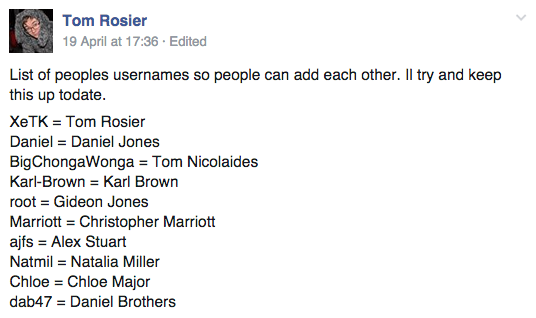
\includegraphics[width=0.75\textwidth]{testing/usernames}
    \caption{The beta test group of users}
    \label{fig:test_users}
\end{figure}

\noindent
A Facebook group was created where the test users could easily raise their concerns with the application and allow a forum for the various individuals to participate in the conversation on how to improve the design of the application and hopefully create a more rounded application for the users to use. Images of the Facebook group can be found in figure \ref{fig:facebook_group}.

\begin{figure}[H]
    \centering
    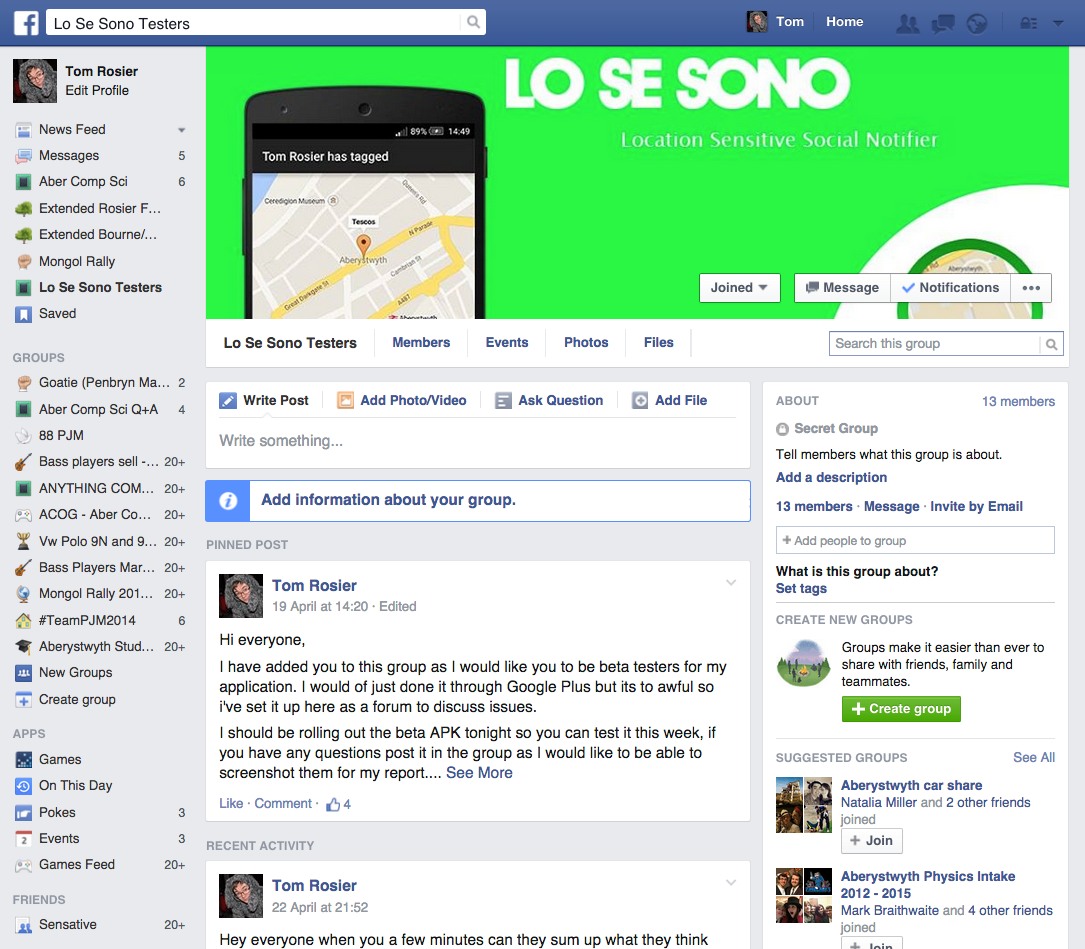
\includegraphics[width=\textwidth]{testing/forum}
    \caption{Facebook used as a forum to voice issues \& feedback}
    \label{fig:facebook_group}
\end{figure} 

\noindent
The test community was used in the very last part of the development when it was felt that the application was nearing a point where it could be used reliably by a reasonably sized group of users. It was pushed out to the group of beta testers for them to test and find issues within the application.\\
\\
It quickly became apparent that there were a number of issues contained within the application that meant that it did not behave correctly. These issues were reported through the Facebook group or GitHub where they could quickly be verified and checked for the authenticity.\\
\\
In figure \ref{fig:gideons_feedback} it shows Gideon Jones raising an issue that a person can be marked in two different places at the same time. If there is a refresh of the items on the screen it will draw the marker in two different distinct places and will lead to a confusing event for the user of the application as they will be unable to tell where the marker will be placed and one is still stuck in the older location.\\
\\
Gideon also queries if the application will log into multiple different devices, which was an aspect that was not made clear to the users of the application. The application has been designed to work on multiple devices at the same time under the same user.

\begin{figure}[H]
    \centering
    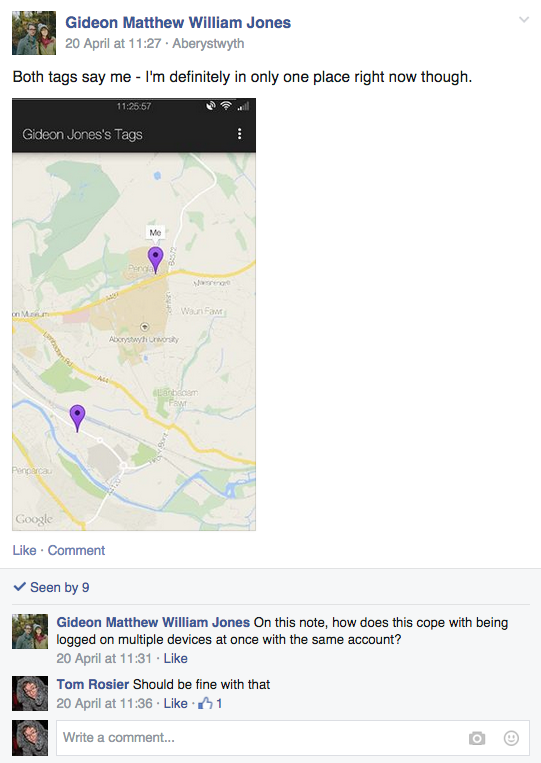
\includegraphics[width=0.75\textwidth]{testing/gideonmultiplepointers}
    \caption{Gideons feedback on issues}
    \label{fig:gideons_feedback}
\end{figure} 

\noindent
Again in figure \ref{fig:toms_feedback} Tom Nicolaides comments on the same issue as Gideon and asks for extra support from the community to verify the issue. He also mentions another issue with the application where it crashes if the GPS is not enabled when the application is initially loaded up, which has been a known issue for a large period of time, but has not impacted development so has yet to be fixed.

\begin{figure}[H]
    \centering
    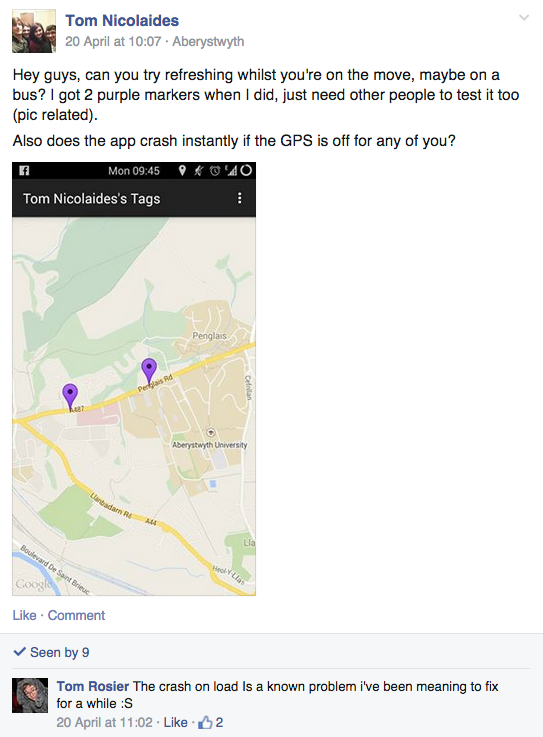
\includegraphics[width=0.75\textwidth]{testing/tommultiplepointers}
    \caption{Tom's feedback on multi location issue}
    \label{fig:toms_feedback}
\end{figure}

\noindent
The use of user based testing was a very helpful way to assess whether the application worked well in the hand of real users and to see if the concept held up as a whole and would be a useful tool for users to use in the real world. From the testing it seems that the concept works and that users do like the functionality given to the end users.

\subsection{Test Devices}

Table \ref{table:device_table} contains a list of devices used to test the application with the various points including model name, Android version, screen resolution, if they are stock or rooted (have been modified), and who owns the device. With this wide array of devices it helped test a large demographic of different devices and different versions of Android. Unfortunately, within the group of users most people tend to have a group of popular devices (mostly Samsung Galaxy devices or HTC One's) where they were very popular devices when they were released and when that group of users purchased their devices they were the best devices to buy.\\
\\
The majority of the devices were running a version of Android Lollipop and had a screen resolution greater than 720p, which made this a good selection of newer devices to work with and they should have a fairly up to date API level that the application can work with. The older Samsung Galaxy S2's and Galaxy Fame were running fairly old software by today's standard and showed some issues due to the lack of some of the newer API's.

\begin{center}
\begin{table}
\begin{tabular}{ l c c c r }
\hline
Device & Android Version & Screen Resolution & Rooted & Owner \\
\hline
Motorola G Gen 1 & 5.0.2 & 1280 x 720 & no & Mark Rosier \\
Motorola G Gen 2 & 5.0.2 & 1280 x 720 & no & Daniel Brothers \\ 
\hline
LG G-Pad 8.3 & 5.0.2 & 1920 x 1200 & yes & Gideon Jones \\
LG Nexus 4 & 5.1 & 1280 x 768 & no & Alex Stuart \\
LG G3 & 5.0 & 2560 x 1440 & no & Joe Roberts \\
\hline
Sony Xperia Z1 Compact & 4.4.2 & 1280 x 720 & no & Chris Marriott \\ 
Sony Xperia Z3 & 5.0.2 & 1920 x 1080 & no & Alex Stuart \\
\hline
Samsung Galaxy S2 & 5.1 & 800x480 & yes & Tom Rosier \\
Samsung Galaxy S2 & 4.1.2 & 800x480 & no & Tom Rosier \\
Samsung Galaxy S2 & 4.1.2 & 800x480 & no & Sam Jackson \\
Samsung Galaxy S3 & 4.4.4 & 1280 x 720 & yes & Tom Nicolaides \\
Samsung Galaxy S3 & 4.3 & 1280 x 720 & no & Daniel Jones \\
Samsung Galaxy S3 & 4.3 & 1280 x 720 & no & Chris Savill \\
Samsung Galaxy Fame & 4.1.2 & 480 x 320 & no & Neil Taylor \\
\hline
HTC One M7 & 4.4.3 & 1920 x 1080 & yes & Gideon Jones \\
HTC One M7 & 4.4.4 & 1920 x 1080 & yes & Karl Brown \\
HTC One M7 & 5.0.2 & 1920 x 1080 & yes & Tom Rosier \\
HTC One M7 & 5.0.2 & 1920 x 1080 & no & Natalia Miller \\
HTC One M8 & 5.0.2 & 1920 x 1080 & no & Chloe Major \\
HTC One M9 & 5.0.2 & 1920 x 1080 & no & Karl Brown \\
\hline
\end{tabular}
\caption{Table of devices used for testing}
\label{table:device_table}
\end{table}
\end{center}

\section{Unit Testing}

Unit testing was used within specific areas of the application, most specifically the backend API, to verify that in fact the RESTful requests are working correctly and are returning the information they should be.\\
\\
Due to the nature of Android it was fairly difficult to unit test the application as everything was very asynchronous and difficult to integrate tests into effectively. With more time and patience it is completely possible to have added in unit tests to the application, but due to early delays and issues the unit testing of these areas got left behind and would definitely need to be added to ensure that the application is working correctly.\\
\\
The Unit tests used to ensure the back end is working correctly focused on the RESTful routes of the application and verified that the changes were made to the application where appropriate or the data being returned was definitely the correct data that the user should be receiving.\\
\\
A list of the tests deployed via unit tests can be found in Appendix \ref{ch:apx_testing} section \ref{sec:test_tables}.

\section{UI Testing}

The other large area of testing carried out was seeing how the UI that had been designed and developed scales to different devices, as the device was primarily developed on a 1080p device. Due to the application only being developed to a proof of concept stage, some of the UI has not been finished to its full potential, so on smaller resolution screens, although some consideration has been made to ensure that the UI elements should fit, as you can see in figures \ref{fig:ui_scaling_home_image}, \ref{fig:ui_scaling_post_image}, \ref{fig:ui_scaling_view_image} and \ref{fig:ui_scaling_friends_image} the UI does not scale correctly with sub 1080p devices. This causes some issues with the usability of the application on these lower resolution devices.\\
\\
These issues would be fixed on newer iterations of the application as there would be more opportunity to design the UI to work on the different resolutions, with special layouts being created to add support for the lower resolution devices. This is covered more in depth in chapter \ref{ch:design} section \ref{sec:development_future_dev}.\\
\\
The UI scaling pictured in figure \ref{fig:ui_scaling_home_image} shows a best case scenario where everything has scaled correctly and the user can see exactly what is going on. The only slight difference is that the user can't quite see as much of the map on the lower resolution devices compared to the other devices.\\
\\
There was feedback from the testing stages that says the home page of the application is fairly hard to understand when coming in new to the application and that some features that should be easily accessible within the UI are not and it should be changed to make it easier to the users to find these functions. This will be changed within further development to help improve the usability of the application overall.

\begin{figure}[H]
    \centering
    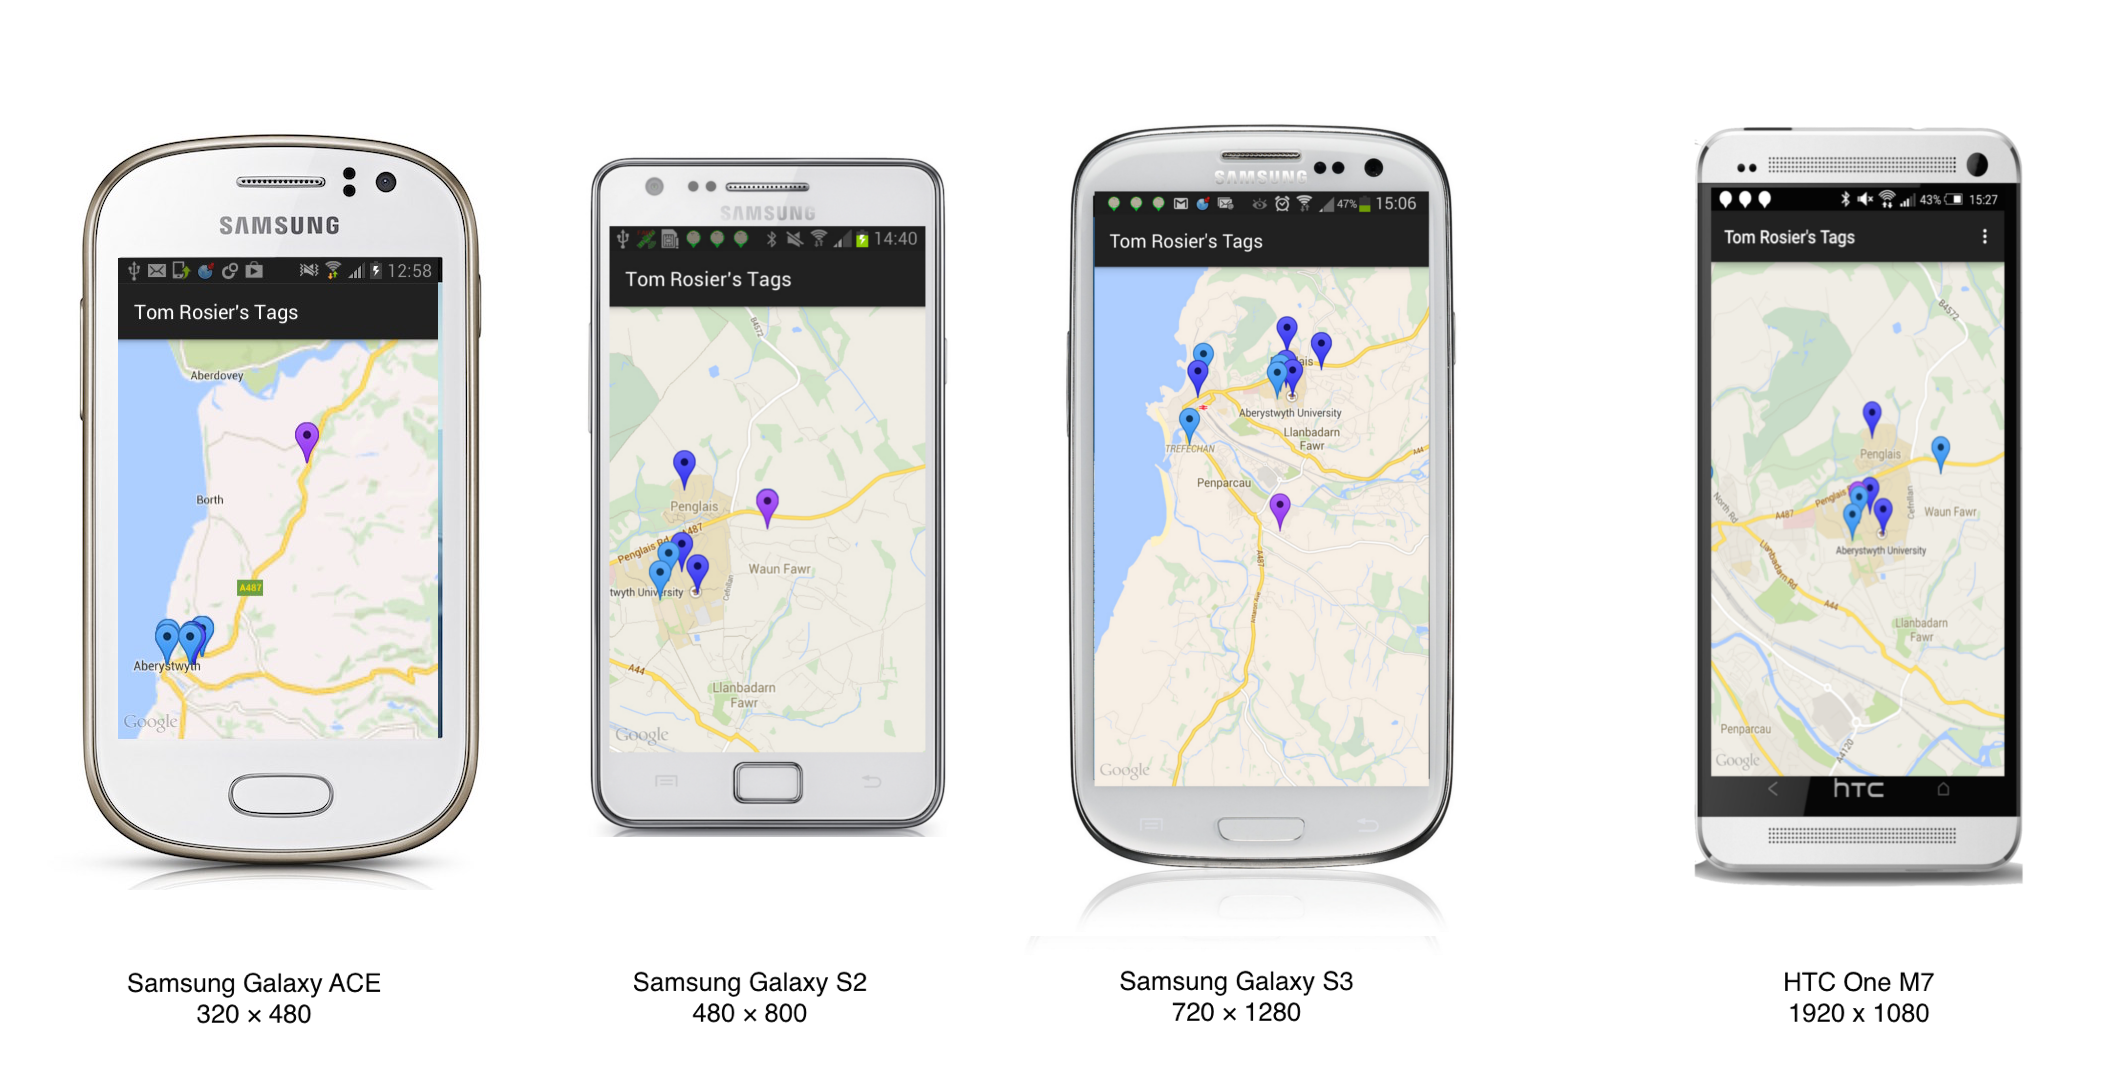
\includegraphics[width=\textwidth]{uiscaling/home}
    \caption{Home activity on different devices}
    \label{fig:ui_scaling_home_image}
\end{figure}

\noindent
The posting messages screen is one of the screens that does not scale as well on a lower resolution device compared to the other pages. It has the issue that the UI elements start to overlap and the lower screen resolution is causing issues in being able to access all of the buttons in the correct places. As you can see in figure \ref{fig:ui_scaling_post_image}, by the time we get to the Galaxy Fame the text field is overlapping the post button which causes an issue, but at least the screen is still functional and the user can still carry out the action that they were intending to do.\\
\\
The posting UI still needs some work to ensure that it can be easily understood by all the users. The UI elements at the current point remain unclear to the user and they tend to need to have to experiment to fully understand what is happening in the UI. This is down to time constraints and with more time the UI will mature to a point where it is much more usable and easy to interpret by the users.

\begin{figure}[H]
    \centering
    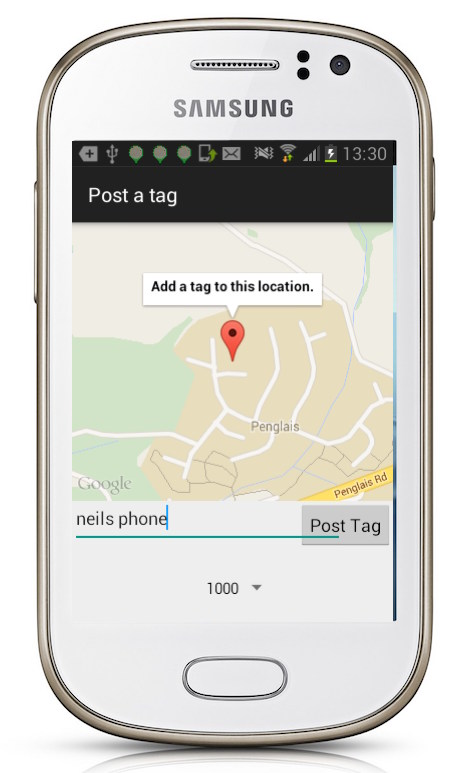
\includegraphics[width=\textwidth]{uiscaling/post}
    \caption{Post message activity on different devices}
    \label{fig:ui_scaling_post_image}
\end{figure} 

\noindent
Viewing of messages is the most complicated screen within the application and surprisingly scales fairly well on most devices, bar the Samsung Galaxy Fame, which came as a shock as there are a lot of UI elements all working together in a fairly confined space. For the smaller screen resolution a new layout would need to be designed to allow everything to be displayed correctly and in a way that is friendly for lower resolution devices. These changes could be made fairly easily and would quickly bring the application to a point where it could be used on all sorts of devices.\\
\\
These problems are caused by the restricted development time of the project and with more time these issues will be resolved. But with the short time given the application stands up fairly well with minimal testing on lower resolution devices.\\
\\
The viewing of messages UI also needs some work to help with its usability. At the current time it looks too cluttered and to be fairly confusing for the user.

\begin{figure}[H]
    \centering
    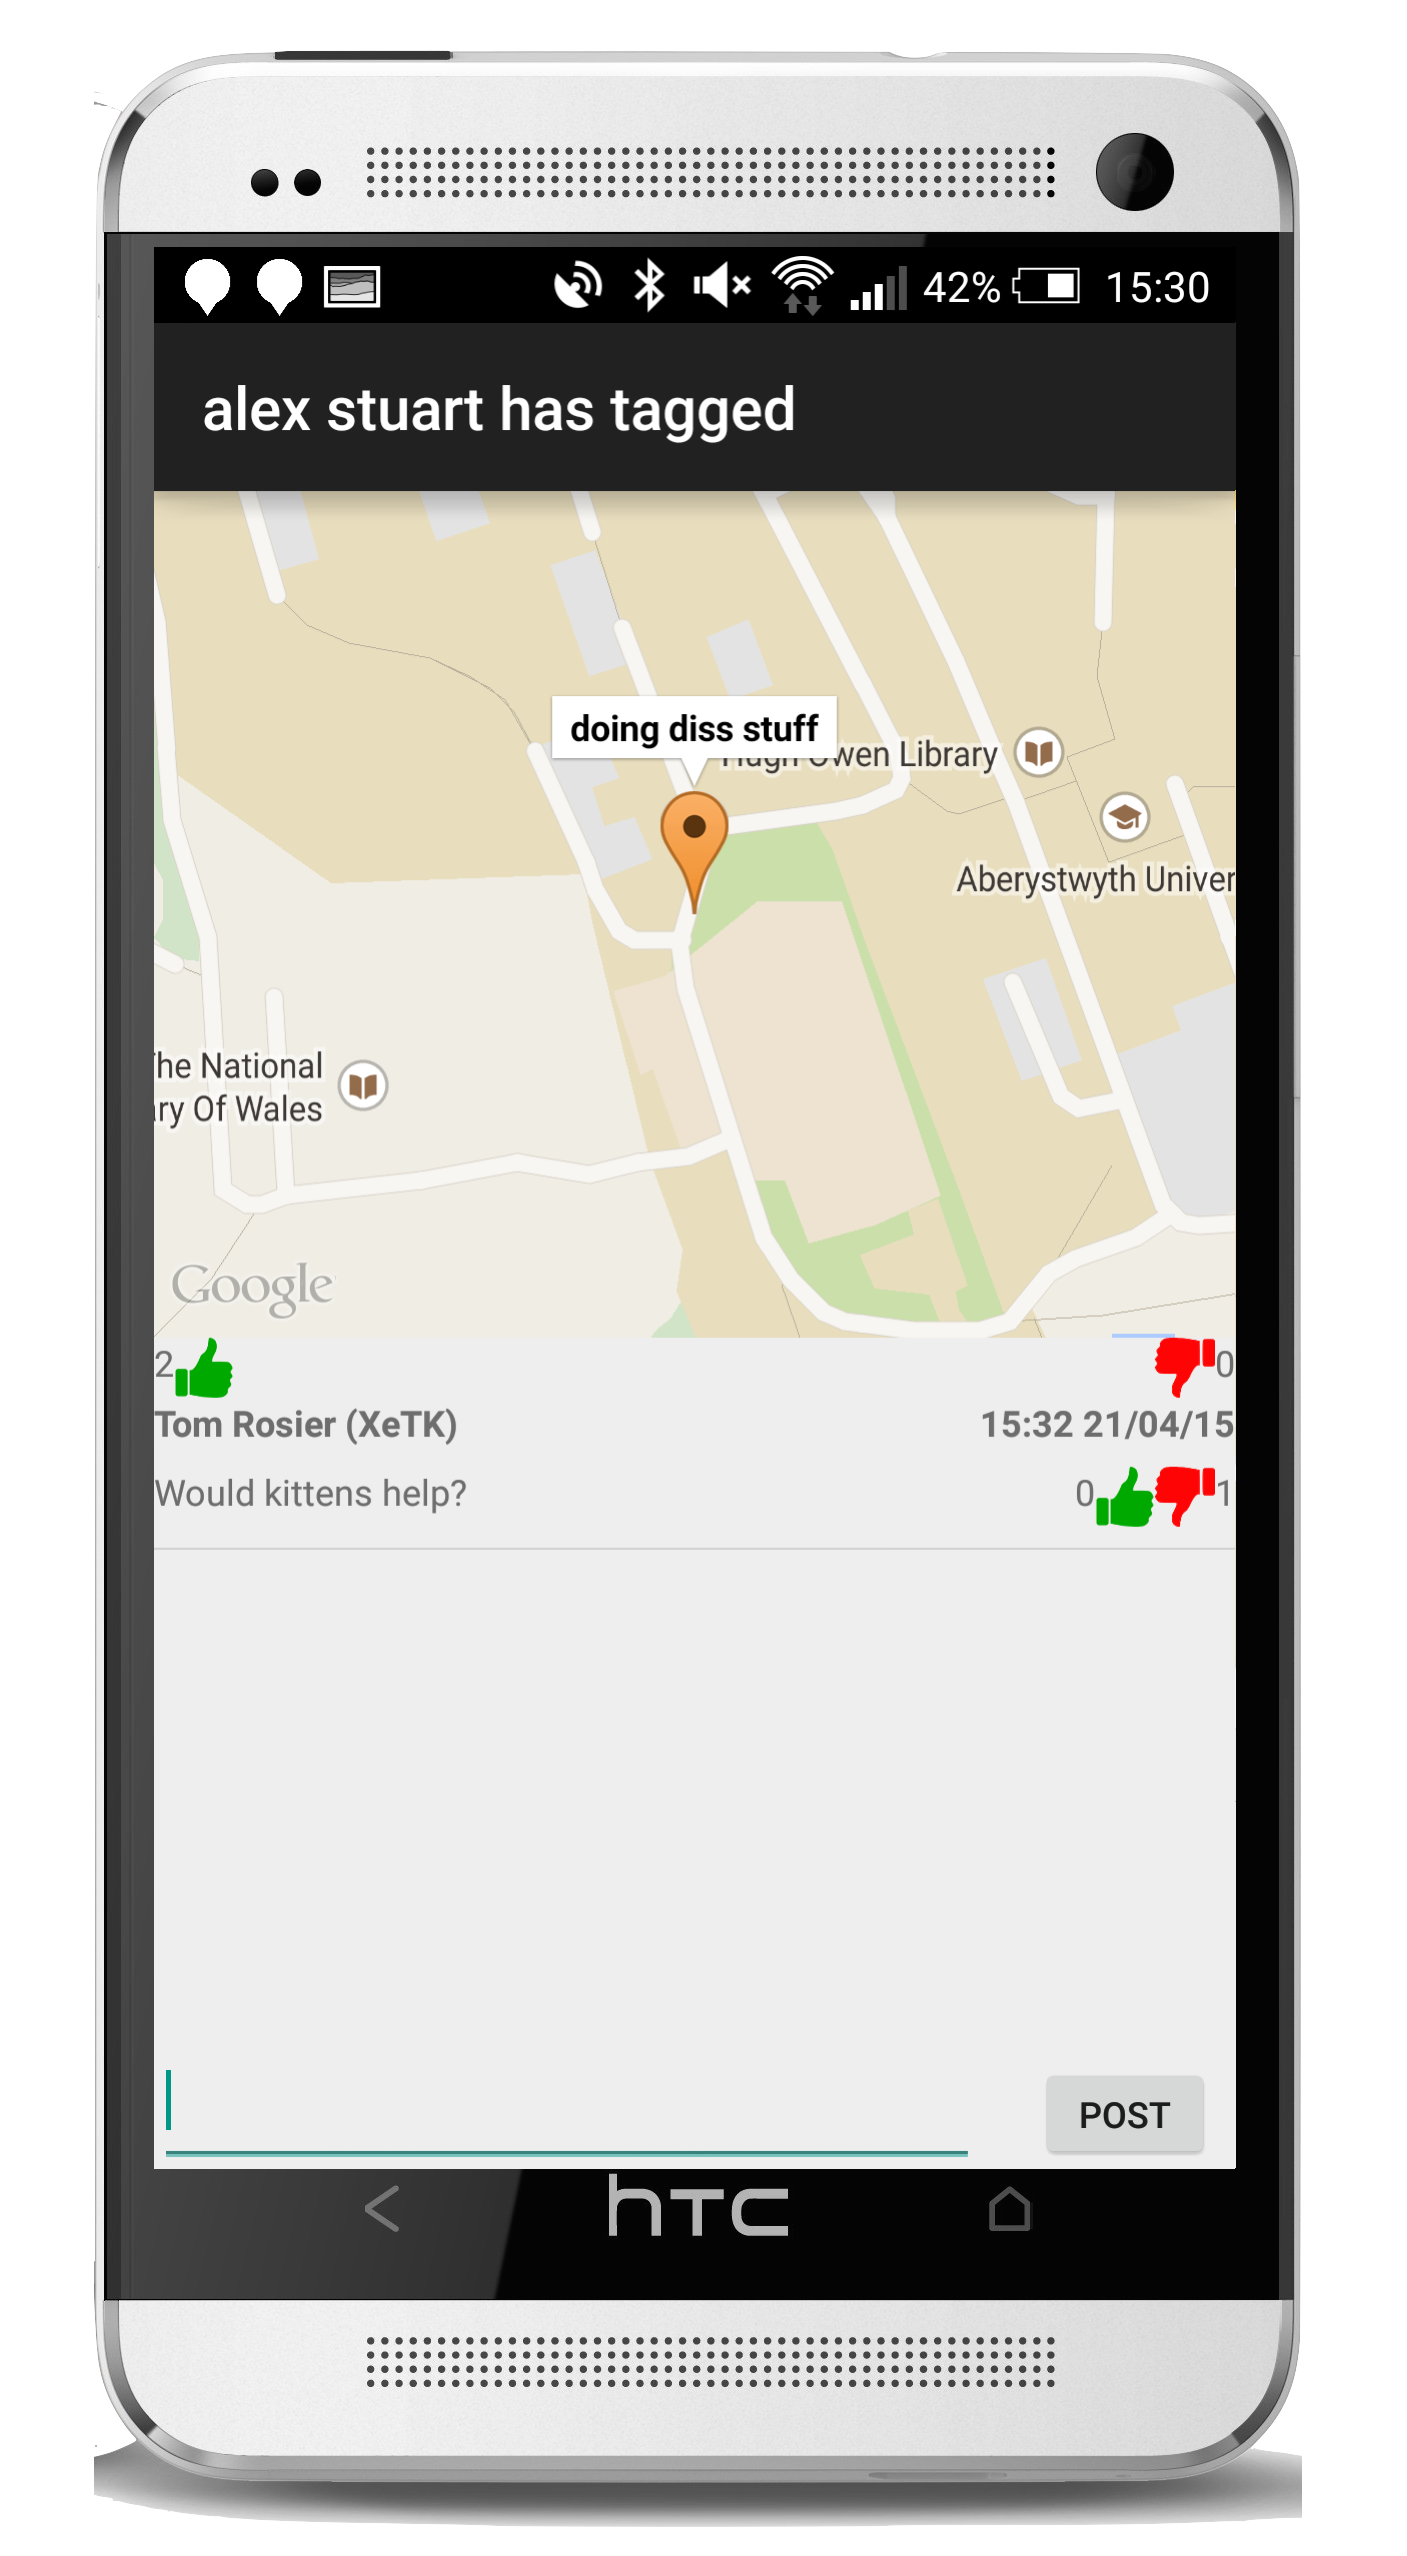
\includegraphics[width=\textwidth]{uiscaling/view}
    \caption{Viewing message on activity on different devices}
    \label{fig:ui_scaling_view_image}
\end{figure} 

\noindent
Due to the screen that adds users to a message being fairly simple, it was possible for it to scale all of the screen sizes easily. It uses a native Android element for the list design, thus there is not much that has been customised for this design, meaning that it should scale fairly effectively to the different UI's.

\begin{figure}[H]
    \centering
    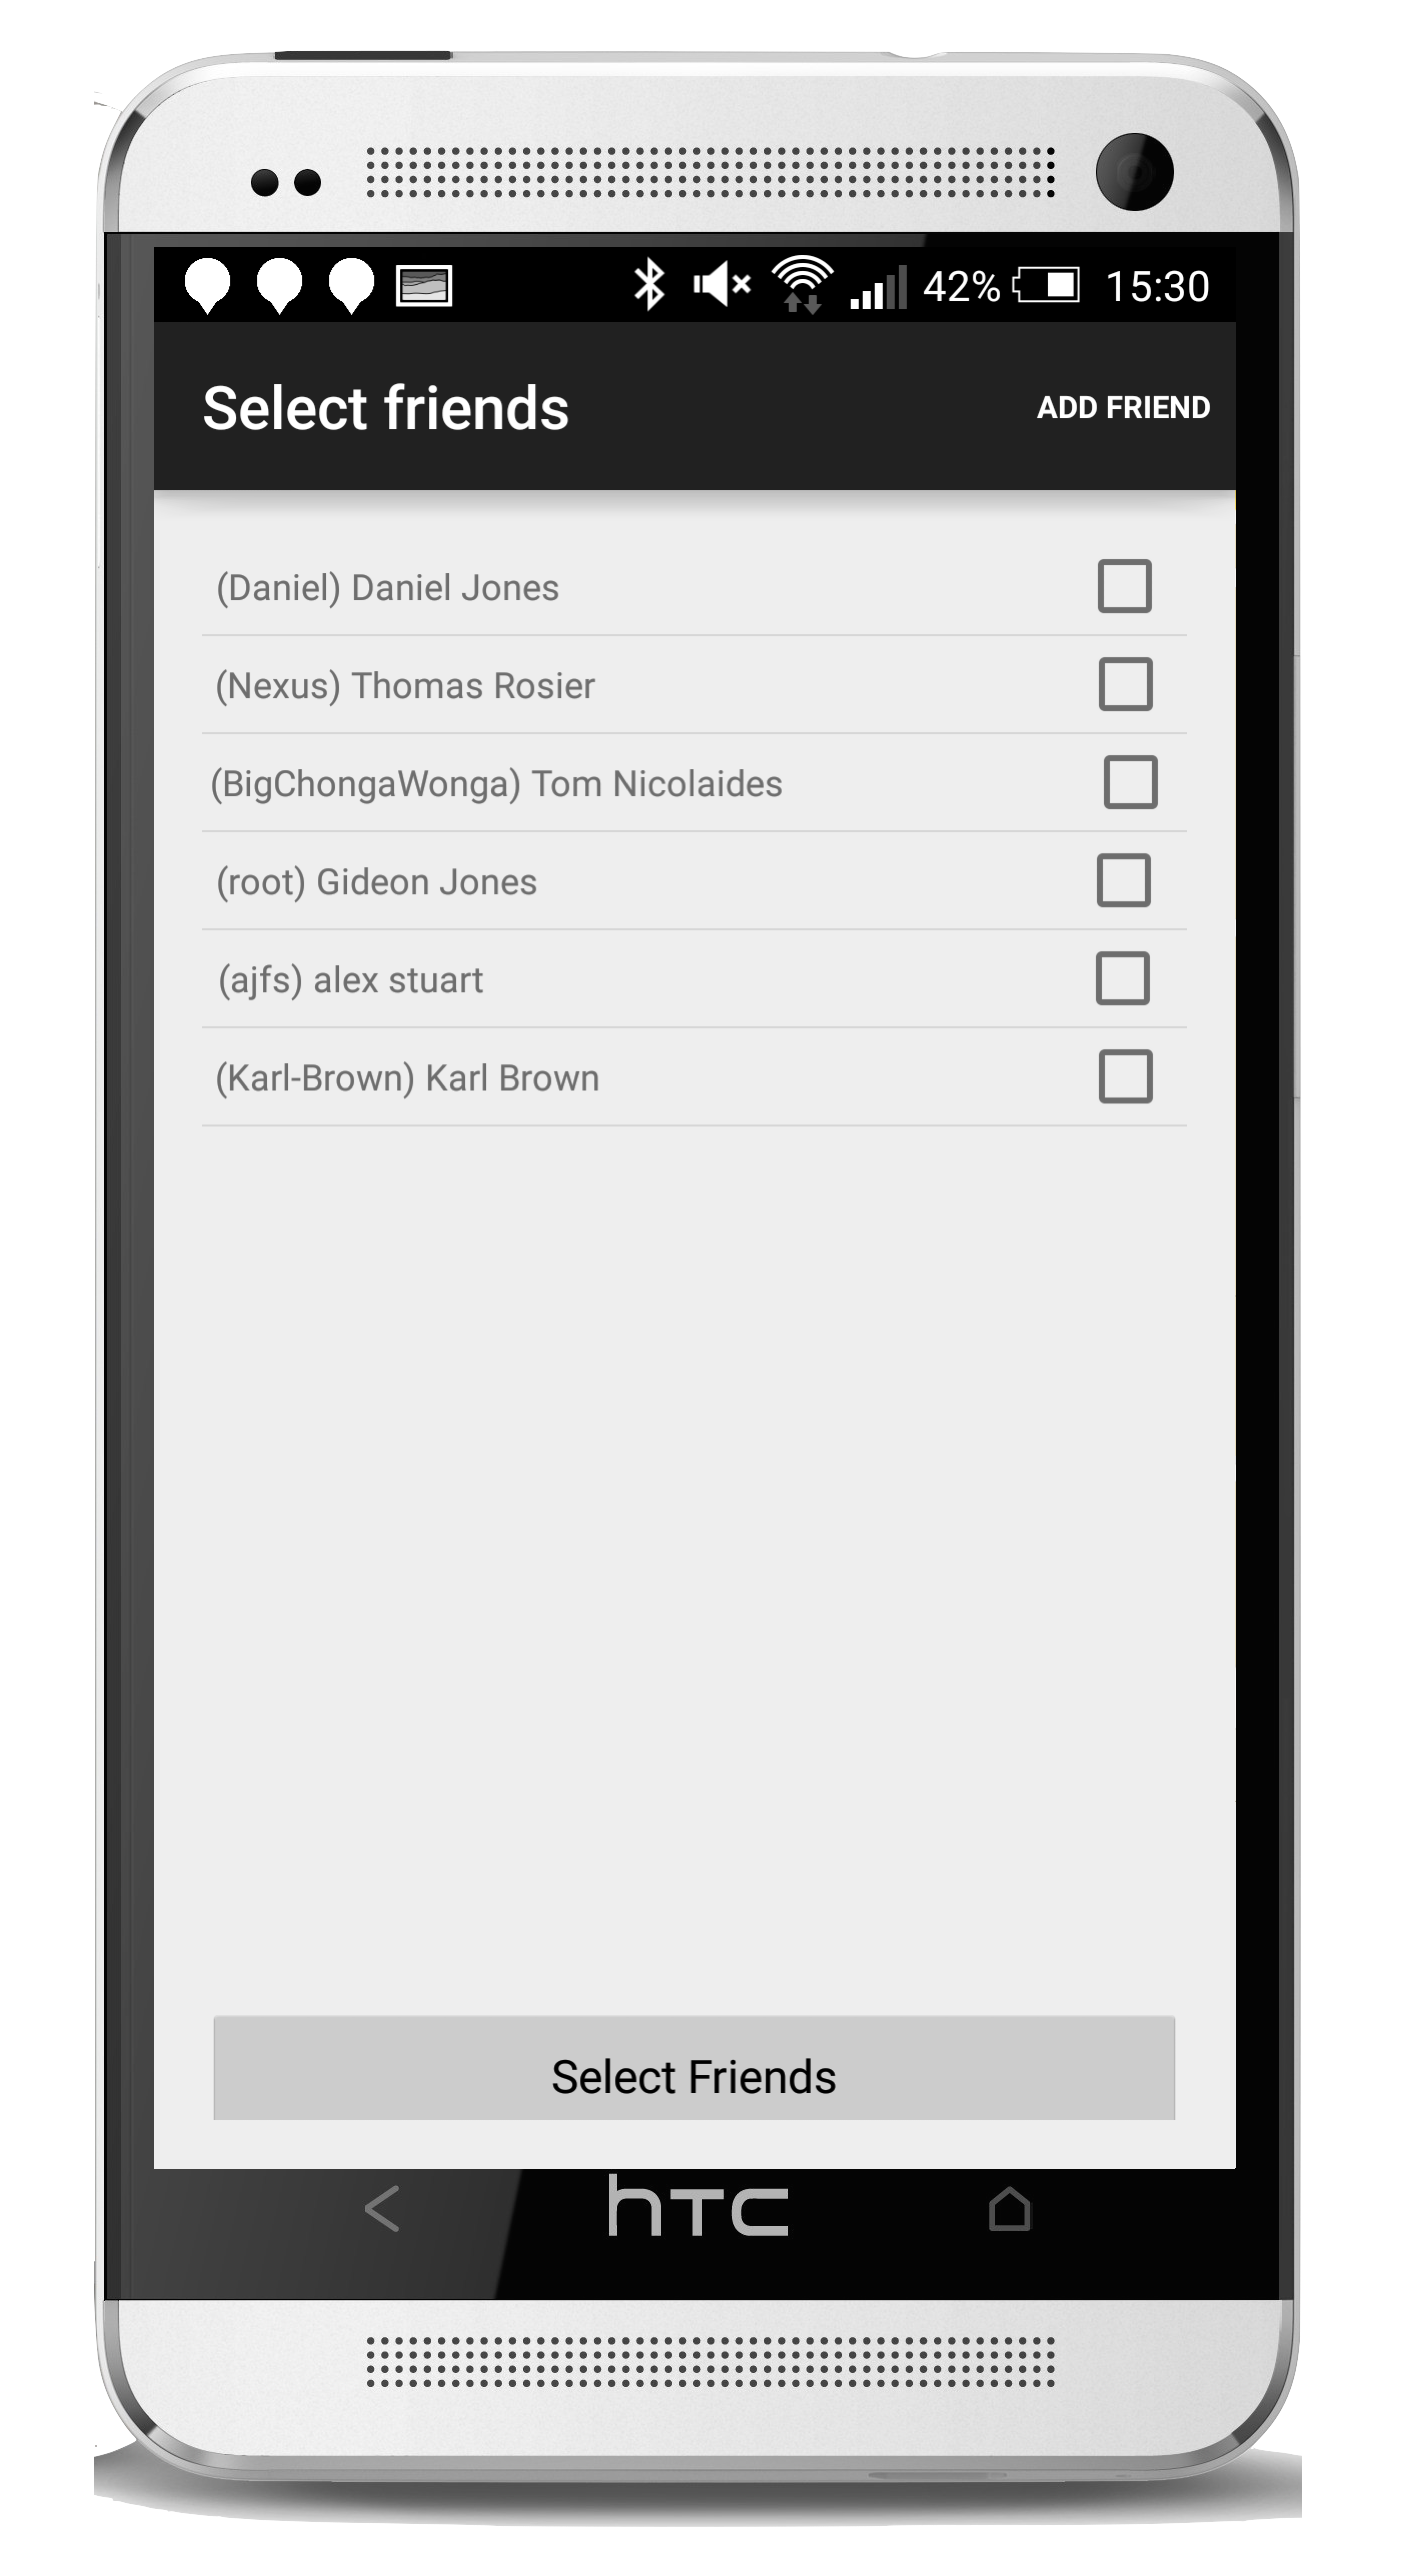
\includegraphics[width=\textwidth]{uiscaling/friends}
    \caption{Setting visibility to friends on different devices}
    \label{fig:ui_scaling_friends_image}
\end{figure} 

\noindent
The UI as it stands currently is usable but it will need more work to get it to a production standard that is expected of an application of this caliber It will require further development to get it to a point where users will want to use the application and some of the oddities of the application will be eradicated.

\section{Functionality Testing}

For each part of the application there is a degree of functionality testing needed to ensure that the application behaves in the correct manor. Each part of the functionally was tested as it was implemented to ensure it would fit in with the requirements needed to make the application work as intended within the functional requirements that were detailed in chapter \ref{ch:design} section \ref{sec:functionality}. This testing was done by the developer of the application as it was developed and development would not move on till it was guaranteed that the application worked in the way expected by the developer to fulfill the functional requirements given for a specific section of the application that is being tested.\\
\\
When the feature was deemed to have completed the testing procedure, development would shift to the next feature in the list of items to develop. The use of user testing along with the testing done by the developer would be enough to deem if the application's functional aspect had reached a level of maturity that suited the feature and if it would work correctly in a production environment. The use of unit testing on the backend application should ensure the robustness of the backend when modifications have occurred to the application to add new functionality into the application. This should mean that the functionality in the backend does not get broken when changes are made.

\section{Stress Testing}

Limited stress testing has been carried out on the application at this point in time. At most there has been 15 users using the application at any given time, which is unlikely to have put a major strain on the system. So far, although there has been issues with the backend application, this seems to originate in the Sequelize library, but more work needs to be undertaken to diagnose where exactly the issue is coming from. For now, allocating more ram to the VPS solves the issue, but it would be preferred to try and fix the issue fully. But again this is a point to cover in future development and not at the current version that the application is in.\\
\\
The user testing has been used to stress out the application screens and ensure that they are robust and will take abuse from the users. Some of the users that are testing the application are fairly technical and have tried various SQL attacks and Overflows to try and break the application. This may be a place where automated testing could be added to test the various parts of the user experience to see if they fall over from various types of attacks, including buffer overflows and SQL injection attacks.\\
\\
Building up the testing suite for the application to ensure that all parts of the application are protected from various malicious attacks and large amounts of data requests, should ensure the application is robust within a production environment. Additionally, it will ensure that the user's experience will be good and they should not be disappointed with the experience provided by the application as a whole.\\
\\
The use of stress testing should ensure the application will have capable error handling, along with being robust, which will ultimately lead to the application being readily available and up for all to use at any time that they want to use it. Work needs to be continued to get the application to this stage, but due to being a proof of concept application the robustness in the application is lacking and more work will be needed to turn the project into a robust product that users want to use.
